\documentclass[12pt]{article}

\usepackage{ceai}
\graphicspath{{../figs/}}

\begin{document}
\doublespacing

\title{CE 488/5588: Applied AI for Engineering\\ \large Topic 16: Modern LLM Systems and Direct Engineering Applications}
\author{}
\date{}
\maketitle

\begin{ch-box}
Topic 15 introduced the motivation for large language models, the historical difficulty of NLP, the rise of transformers, tokenization, embeddings, vector spaces, vector stores, and the basic limits of probabilistic generation. This chapter moves one step closer to practice. The central question is no longer only ``what is an LLM?'' but ``how are modern LLM systems actually organized, and how are they already changing engineering work before full agentic AI?''
\end{ch-box}

\section*{Learning Objectives}
After completing this chapter, you should be able to:
\begin{itemize}
    \item distinguish encoder-only, decoder-only, and encoder-decoder transformer families at a high level;
    \item explain the difference between a base model and a post-trained assistant;
    \item describe prompt engineering as workflow design rather than as a single clever prompt;
    \item explain how retrieval-augmented generation (RAG), LangChain-style pipelines, and knowledge graphs support engineering knowledge systems;
    \item describe first-generation LLM engineering patterns such as structured prompting and ReAct; and
    \item explain why these workflows naturally lead into the frontier topic of agentic AI and human-in-the-loop engineering.
\end{itemize}

\section{From Topic 15 to Topic 16}

Topic 15 focused on representation: how text becomes tokens, how tokens become vectors, and how vectors enable semantic retrieval. Topic 16 now focuses on \emph{systems}. An LLM used in practice is rarely just a raw pretrained neural network. It is usually part of a larger workflow that includes prompt design, post-training, retrieval, formatting rules, external tools, and user supervision.

This distinction matters in engineering. A language model can produce fluent text on its own, but a usable engineering assistant usually needs structure: relevant documents, source traceability, task decomposition, and a clear boundary between what is generated and what must be verified.

\begin{alert-box}
\textbf{Scope decision for this chapter:} Topic 16 focuses on direct LLM applications and first-generation LLM engineering. It introduces structured prompting, RAG, LangChain-style orchestration, knowledge-graph construction, and ReAct-style workflows. Full frontier agentic workflows, skills, and autonomous research systems are reserved for Topic 17.
\end{alert-box}

\subsection{Why LLM Systems Are More Than Chatbots}

The public often encounters LLMs through a chat window, but the engineering reality is broader. A useful deployed system usually combines several layers: a model architecture, post-training, prompting structure, retrieval or tool use, and human supervision. In that sense, Topic 16 is not merely about another model family. It is about the system stack that turns a language model into an engineering assistant.

\begin{figure}[ht]
    \centering
    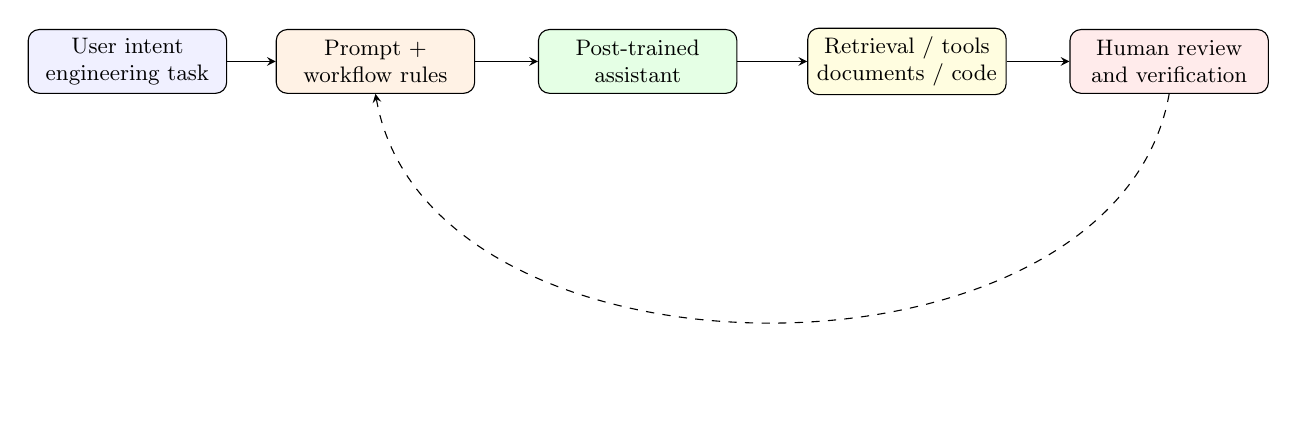
\begin{tikzpicture}[>=stealth,font=\small, scale=0.90, transform shape]
        \tikzset{box/.style={draw, rounded corners, minimum width=2.8cm, minimum height=0.9cm, align=center}}
        \node[box, fill=blue!6] (user) at (0,0) {User intent\\engineering task};
        \node[box, fill=orange!10] (prompt) at (3.5,0) {Prompt +\\workflow rules};
        \node[box, fill=green!10] (assist) at (7.2,0) {Post-trained\\assistant};
        \node[box, fill=yellow!12] (tools) at (11.0,0) {Retrieval / tools\\documents / code};
        \node[box, fill=red!8] (verify) at (14.7,0) {Human review\\and verification};
        \draw[->] (user) -- (prompt);
        \draw[->] (prompt) -- (assist);
        \draw[->] (assist) -- (tools);
        \draw[->] (tools) -- (verify);
        \draw[dashed,->] (verify.south) to[out=-100,in=-80] (prompt.south);
    \end{tikzpicture}
    \caption{A practical system view of an engineering LLM assistant. In real use, the model sits inside a larger workflow that includes prompting, tools, retrieved evidence, and human verification.}
    \label{t16fig:system_stack}
\end{figure}

This broader system view is also what connects Topic 16 back to Topic 15. Topic 15 explained why embeddings, retrieval, and probabilistic generation matter. Topic 16 asks how those ingredients are assembled into practical systems that can support real work.

\section{Mainstream Architectures of Modern LLM Systems}

Although the public often speaks of ``LLMs'' as if they were one architecture, transformer-based language systems come in several important families.

\subsection{Encoder-Only Models}

Encoder-only models, such as BERT-style systems, process input with bidirectional attention. Every token can attend to the full input sequence. This makes encoder-only systems strong for representation tasks such as classification, semantic similarity, retrieval, and embedding generation.

A common pretraining objective for encoder-style models is masked-token prediction:
\begin{equation}
    \mathcal{L}_{\mathrm{MLM}}(\theta)
    = -\sum_{t\in \mathcal{M}} \log P_\theta(x_t \mid x_{\setminus t}),
    \label{t16eq:mlm}
\end{equation}
where $\mathcal{M}$ denotes the set of masked positions.

The practical point is that encoder-only models are excellent when the output is primarily an internal representation rather than open-ended generation.

\subsection{Decoder-Only Models}

Decoder-only models, such as GPT-style systems, use causal attention. Each token sees only the tokens before it. This architecture is the dominant backbone for modern general-purpose chat and coding assistants because it matches the autoregressive generation process naturally:
\begin{equation}
    P(x_1,\dots,x_T) = \prod_{t=1}^T P(x_t\mid x_{<t}).
    \label{t16eq:autoregressive}
\end{equation}

Decoder-only systems became dominant largely because they are simple to scale and unify many tasks under one objective. In practice, if students interact with a large conversational assistant, they are usually interacting with a decoder-only or mostly decoder-centered system.

\subsection{Encoder-Decoder Models}

Encoder-decoder systems, such as T5-style sequence-to-sequence models, split processing into two stages. The encoder builds a representation of the source input, and the decoder generates the target sequence using both causal self-attention and cross-attention to the encoder output. The conditional objective has the form
\begin{equation}
    P(y\mid x) = \prod_{t=1}^{T_y} P(y_t \mid y_{<t}, x).
    \label{t16eq:seq2seq}
\end{equation}

This design is especially natural for translation, summarization, structured transformation, and other tasks where the input and output play clearly different roles.

\begin{table}[ht]
    \centering
    \caption{A practical comparison of the three transformer families.}
    \label{t16tab:architectures}
    \begin{tabulary}{\textwidth}{L L L}
        \toprule
        \textbf{Architecture} & \textbf{Strength} & \textbf{Typical use} \\
        \midrule
        Encoder-only & rich bidirectional representation & embeddings, classification, retrieval \\
        Decoder-only & scalable generation from prompts & chat, coding, general assistants \\
        Encoder-decoder & explicit input-to-output mapping & translation, summarization, structured generation \\
        \bottomrule
    \end{tabulary}
\end{table}

\begin{ex-box}
\textbf{Engineering interpretation.} If you want to embed inspection reports for search, an encoder-style system is natural. If you want a coding or analysis assistant, a decoder-only system is natural. If you want to convert technical descriptions into another textual format, such as summarization or structured reporting, an encoder-decoder design is often conceptually clean.
\end{ex-box}

\subsection{Why Decoder-Only Models Dominated the Public Interface}

The public AI wave after 2020 was largely driven by decoder-only models because they turned one architecture into many products: chat, code completion, summarization, drafting, transformation, and question answering. This was not because encoder-only or encoder-decoder models became useless. Rather, decoder-only systems became the most versatile general front end.

\begin{figure}[ht]
    \centering
    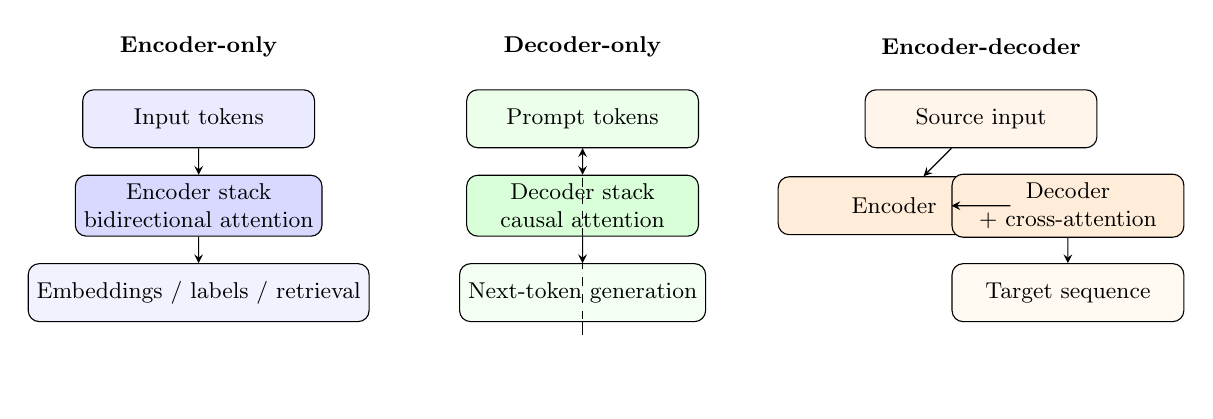
\begin{tikzpicture}[>=stealth,font=\small, scale=0.92, transform shape]
        \tikzset{box/.style={draw, rounded corners, minimum width=3.2cm, minimum height=0.8cm, align=center}}

        \node[box, fill=blue!8] (encin) at (0,2.0) {Input tokens};
        \node[box, fill=blue!15] (enc) at (0,0.8) {Encoder stack\\bidirectional attention};
        \node[box, fill=blue!5] (encout) at (0,-0.4) {Embeddings / labels / retrieval};
        \draw[->] (encin) -- (enc);
        \draw[->] (enc) -- (encout);

        \node at (0,3.0) {\textbf{Encoder-only}};

        \node[box, fill=green!8] (decin) at (5.3,2.0) {Prompt tokens};
        \node[box, fill=green!15] (dec) at (5.3,0.8) {Decoder stack\\causal attention};
        \node[box, fill=green!5] (decout) at (5.3,-0.4) {Next-token generation};
        \draw[->] (decin) -- (dec);
        \draw[->] (dec) -- (decout);
        \draw[dashed,->] (decout.south) to[out=-90,in=-90] (decin.south);

        \node at (5.3,3.0) {\textbf{Decoder-only}};

        \node[box, fill=orange!8] (seqin) at (10.8,2.0) {Source input};
        \node[box, fill=orange!15] (seqenc) at (9.6,0.8) {Encoder};
        \node[box, fill=orange!15] (seqdec) at (12.0,0.8) {Decoder\\+ cross-attention};
        \node[box, fill=orange!5] (seqout) at (12.0,-0.4) {Target sequence};
        \draw[->] (seqin) -- (seqenc);
        \draw[->] (seqenc) -- (seqdec);
        \draw[->] (seqdec) -- (seqout);

        \node at (10.8,3.0) {\textbf{Encoder-decoder}};
    \end{tikzpicture}
    \caption{Three mainstream transformer families. Encoder-only models emphasize representation, decoder-only models emphasize autoregressive generation, and encoder-decoder models emphasize explicit input-to-output transformation.}
    \label{t16fig:transformer_family}
\end{figure}

Figure~\ref{t16fig:transformer_family} is more useful here than a single generic transformer schematic because Topic 16 is about system choices. Students need to see not just that these models all descend from the transformer, but that they support different engineering tasks for structural reasons.

\section{Base Models, Post-Training, and Assistant Behavior}

In Topic 15, we already introduced pretraining, supervised fine-tuning, RLHF, DPO, and LoRA at a foundational level. Here we place those ideas into a more practical system view.

\subsection{Base Model versus Assistant}

A \textbf{base model} is the raw language model after pretraining or after general-purpose training. It has broad competence but may not respond in the way users expect. A \textbf{post-trained assistant} is the result of adding behavioral shaping so that the system follows instructions, answers more helpfully, formats outputs more reliably, and often refuses unsafe requests.

From an engineering perspective, the most important distinction is this: what users experience is not just the architecture. It is the architecture \emph{plus} post-training.

\subsection{Instruction Tuning}

Instruction tuning uses prompt-response demonstrations to help the model follow tasks more directly. If the training set is $\mathcal{D}$, the supervised objective is
\begin{equation}
    \mathcal{L}_{\mathrm{SFT}}(\theta) = -\sum_{(x,y)\in\mathcal{D}} \log P_\theta(y\mid x).
    \label{t16eq:sft}
\end{equation}

This step makes the difference between ``a model that can continue text'' and ``a model that behaves like an assistant.''

\subsection{Preference Optimization}

Not every desired property is a single correct answer. Helpfulness, tone, clarity, professionalism, and concision are often preference-like rather than absolute. This motivates preference learning.

RLHF uses human preferences to train a reward signal and then optimize the model under that signal. DPO simplifies this picture by using preferred and non-preferred outputs more directly. The exact mathematics can be postponed, but students should remember the conceptual shift: from predicting text to optimizing for outputs people prefer.

\begin{def-box}
\textbf{Practical summary.} Pretraining gives general competence. Instruction tuning gives task-following behavior. Preference optimization shapes style, alignment, and subjective quality. Together they explain why a deployed assistant feels different from a raw language model.
\end{def-box}

\subsection{Parameter-Efficient Customization}

Organizations often want to adapt a model without retraining every parameter. This is where methods such as LoRA become useful. Rather than updating the full model, one updates a small number of additional trainable components. This is attractive because it reduces memory cost, engineering complexity, and deployment friction.

For engineering organizations, this matters because many use cases are narrow: internal style guides, project-specific terminology, report templates, compliance phrasing, or domain-focused code assistance. Those use cases may not require a full-model retraining strategy.

\section{First-Generation LLM Engineering Workflows}

Before frontier autonomous agents became a mainstream topic, many practical LLM workflows already existed. These are best understood as \emph{first-generation AI engineering patterns}: more structured than ordinary chat, but not yet full autonomous agents.

\subsection{ReAct as a Bridge Pattern}

One influential pattern is \textbf{ReAct}, short for \emph{reasoning and acting}. The idea is to interleave a short reasoning trace with an action such as search, retrieval, or tool use. In stylized form, the loop looks like this:
\begin{equation}
    \text{Thought} \rightarrow \text{Action} \rightarrow \text{Observation} \rightarrow \text{Thought} \rightarrow \cdots
    \label{t16eq:react}
\end{equation}

ReAct is important pedagogically because it sits between plain prompting and full agentic systems. It shows students that an LLM workflow can be iterative, tool-aware, and partially self-correcting without requiring a fully autonomous platform.

\begin{figure}[ht]
    \centering
    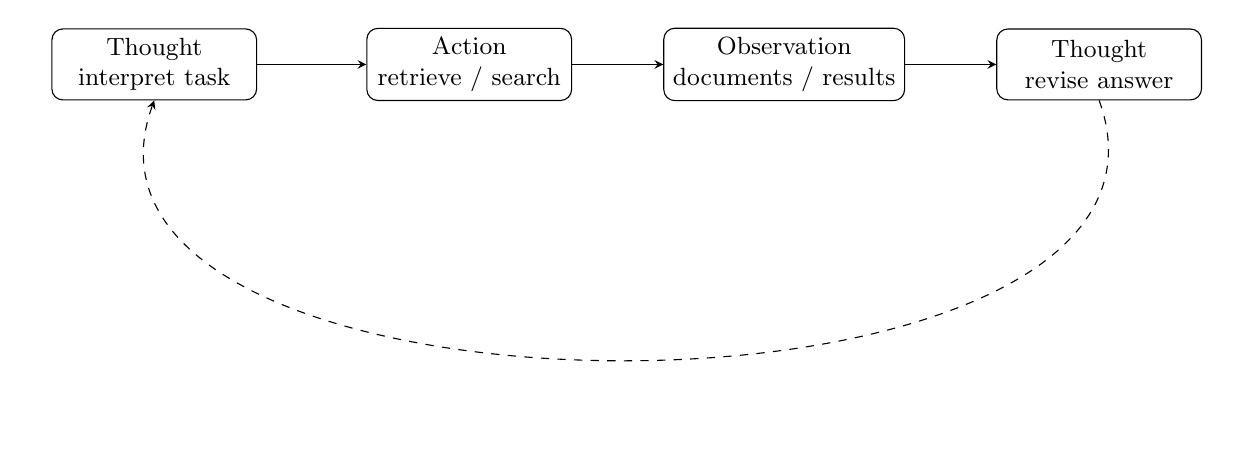
\begin{tikzpicture}[>=stealth,font=\small]
        \tikzset{box/.style={draw, rounded corners, minimum width=2.6cm, minimum height=0.9cm, align=center}}
        \node[box] (t1) at (0,0) {Thought\\interpret task};
        \node[box] (a1) at (4,0) {Action\\retrieve / search};
        \node[box] (o1) at (8,0) {Observation\\documents / results};
        \node[box] (t2) at (12,0) {Thought\\revise answer};
        \draw[->] (t1) -- (a1);
        \draw[->] (a1) -- (o1);
        \draw[->] (o1) -- (t2);
        \draw[dashed,->] (t2.south) to[out=-70,in=-110] (t1.south);
    \end{tikzpicture}
    \caption{A simplified ReAct-style loop. This pattern interleaves reasoning, external action, and observation, making the workflow more structured than ordinary chat while still short of a fully autonomous agent system.}
    \label{t16fig:react}
\end{figure}

\subsection{Why ReAct Matters in Engineering}

Engineering tasks rarely succeed from a single fluent response. The useful process is often iterative: identify the missing source, retrieve the clause, inspect the evidence, revise the conclusion, and document the assumptions. ReAct-style prompting therefore matters because it teaches the model to work with intermediate evidence rather than only to produce an immediate final answer.

\begin{ex-box}
\textbf{Example: code-compliance question.} A user asks, ``What serviceability deflection limit applies here?'' A ReAct-style workflow might first retrieve the relevant code section, then observe that the clause depends on occupancy or finish sensitivity, then ask for or infer that missing context before drafting a bounded answer.
\end{ex-box}

\section{RAG and Knowledge Bases}

Topic 15 introduced vector stores and semantic retrieval. Topic 16 now places them into the practical architecture of a modern engineering assistant.

\subsection{RAG as a System Pattern}

Retrieval-augmented generation (RAG) combines two ideas:
\begin{enumerate}
    \item retrieve relevant external documents; and
    \item condition the generation on those retrieved documents.
\end{enumerate}

The system-level logic can be summarized as
\begin{equation}
    \text{query} \rightarrow \text{retriever} \rightarrow \text{context} \rightarrow \text{generator} \rightarrow \text{answer}.
    \label{t16eq:rag}
\end{equation}

RAG matters because it changes the question from ``What does the model remember?'' to ``What evidence can the system retrieve and use?'' For engineering use, that shift is crucial.

\begin{figure}[ht]
    \centering
    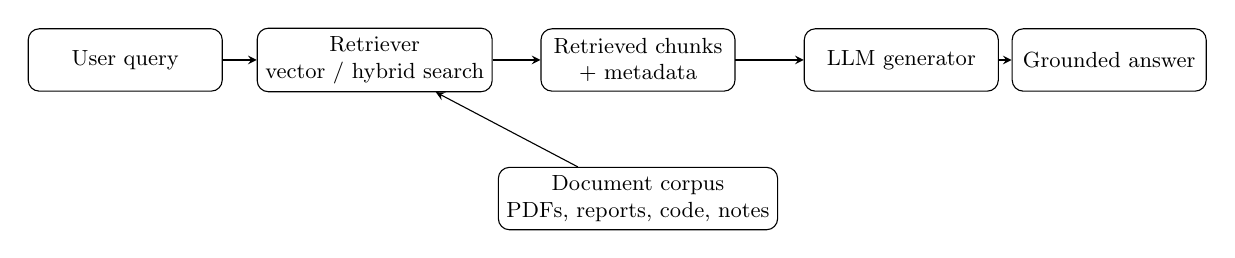
\begin{tikzpicture}[>=stealth,font=\small, scale=0.88, transform shape]
        \tikzset{box/.style={draw, rounded corners, minimum width=2.8cm, minimum height=0.9cm, align=center}}
        \node[box] (q) at (0,0) {User query};
        \node[box] (r) at (3.6,0) {Retriever\\vector / hybrid search};
        \node[box] (d) at (7.4,0) {Retrieved chunks\\+ metadata};
        \node[box] (g) at (11.2,0) {LLM generator};
        \node[box] (a) at (14.2,0) {Grounded answer};
        \draw[->] (q) -- (r);
        \draw[->] (r) -- (d);
        \draw[->] (d) -- (g);
        \draw[->] (g) -- (a);
        \node[box] (c) at (7.4,-2.0) {Document corpus\\PDFs, reports, code, notes};
        \draw[->] (c) -- (r);
    \end{tikzpicture}
    \caption{A practical RAG pipeline for engineering knowledge work. The retriever brings relevant chunks and metadata into the context window before generation, so the answer depends on accessible evidence rather than only model memory.}
    \label{t16fig:rag}
\end{figure}

\subsection{LangChain-Style Orchestration}

Frameworks such as LangChain became popular not because they changed the mathematics of language models, but because they made it easier to connect prompts, retrievers, tools, memory, and output formatting into one workflow. In other words, they are orchestration layers for LLM applications.

For students, the important concept is not any one framework API. It is the architectural pattern:
\begin{itemize}
    \item prompt template;
    \item retriever or database connector;
    \item LLM call;
    \item parser or structured output step; and
    \item optional memory or tool integration.
\end{itemize}

This is why one can use LangChain or a similar framework to build an engineering knowledge assistant without yet building a full agent.

\subsection{Engineering Knowledge Bases}

A useful engineering knowledge base is not just a pile of text. It is an indexed, chunked, traceable corpus with metadata, version awareness, and often domain-specific filtering. For example, a structural engineering knowledge base may need to separate design codes, office standards, project memos, spreadsheets, and prior report sections.

The technical challenge is not merely retrieval quality. It is also governance: which source is official, which is superseded, and which may only be advisory.

\begin{figure}[ht]
    \centering
    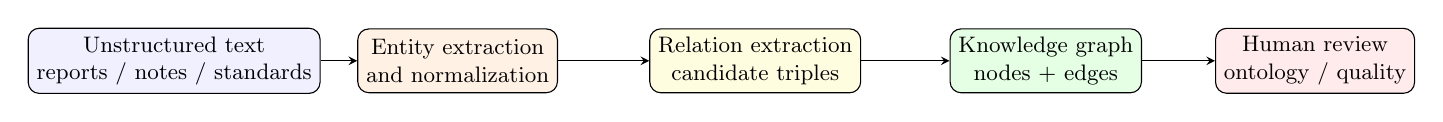
\begin{tikzpicture}[>=stealth,font=\small, scale=0.90, transform shape]
        \tikzset{box/.style={draw, rounded corners, minimum width=2.7cm, minimum height=0.9cm, align=center}}
        \node[box, fill=blue!6] (text) at (0,0) {Unstructured text\\reports / notes / standards};
        \node[box, fill=orange!10] (entity) at (4.0,0) {Entity extraction\\and normalization};
        \node[box, fill=yellow!12] (relation) at (8.2,0) {Relation extraction\\candidate triples};
        \node[box, fill=green!10] (graph) at (12.3,0) {Knowledge graph\\nodes + edges};
        \node[box, fill=red!8] (review) at (16.1,0) {Human review\\ontology / quality};
        \draw[->] (text) -- (entity);
        \draw[->] (entity) -- (relation);
        \draw[->] (relation) -- (graph);
        \draw[->] (graph) -- (review);
    \end{tikzpicture}
    \caption{A simplified text-to-knowledge-graph workflow. LLMs can assist with extracting entities and relations, but the resulting graph still requires normalization and human review.}
    \label{t16fig:kg_pipeline}
\end{figure}

\section{Knowledge Graph Creation with LLMs}

RAG is not the only way to organize knowledge. Another important direction is to use LLMs to help build or extend \textbf{knowledge graphs}.

\subsection{Why Knowledge Graphs Matter}

A knowledge graph stores entities and relations explicitly. In a simplified form, one may represent facts as triples:
\begin{equation}
    (h,r,t),
    \label{t16eq:triple}
\end{equation}
where $h$ is the head entity, $r$ is the relation, and $t$ is the tail entity.

For example:
\[
    (\texttt{ACI318},\ \texttt{defines},\ \texttt{load\ combination})
\]
or
\[
    (\texttt{Beam\ B12},\ \texttt{uses\ material},\ \texttt{A992\ steel}).
\]

This is attractive in engineering because graphs support explicit relationships, queryability, and rule-based augmentation.

\subsection{How LLMs Help Build Graphs}

An LLM can assist with graph creation by:
\begin{itemize}
    \item extracting entities from documents;
    \item extracting candidate relations;
    \item normalizing terms to an ontology or vocabulary;
    \item resolving aliases and abbreviations; and
    \item producing draft triples for later human review.
\end{itemize}

The practical lesson is that LLMs can help transform messy engineering text into more structured knowledge artifacts. However, that output must still be reviewed, because an incorrect triple may look formally clean while remaining semantically wrong.

\begin{alert-box}
\textbf{RAG and knowledge graphs are complementary.} RAG is strong when one wants grounded access to source passages. Knowledge graphs are strong when one wants explicit relationships, schema, and structured queries. Many useful engineering systems may combine both.
\end{alert-box}

\section{Prompt Engineering as Workflow Design}

Prompt engineering is sometimes presented as if it were the art of discovering one magical sentence. That is not the most useful engineering view. A better view is that prompt engineering is the design of a \emph{workflow interface} between human intent and model behavior.

\subsection{Prompt Components}

A reliable prompt often specifies several elements explicitly:
\begin{itemize}
    \item \textbf{role:} what the model should act as;
    \item \textbf{context:} what information the model should use;
    \item \textbf{task:} what the model is being asked to do;
    \item \textbf{constraints:} format, scope, tone, or assumptions; and
    \item \textbf{verification cues:} how the model should check itself or cite sources.
\end{itemize}

The reason this works is not mystical. A prompt is effectively a lightweight program written in natural language. It constrains the space of plausible continuations.

\subsection{A Minimal Prompt Template}

For many engineering uses, a compact prompt template is enough:
\begin{verbatim}
Role: You are a structural engineering assistant.
Context: Use only the attached design note and cited code clauses.
Task: Summarize the controlling assumptions for serviceability checks.
Constraints: Return 5 bullet points and cite the source section for each.
Verification: If a needed source is missing, say so explicitly.
\end{verbatim}

This is already a workflow. It tells the model what to do, what not to do, and how to signal uncertainty.

\subsection{Structured Prompting Patterns}

Several prompting patterns are especially useful in practice:
\begin{itemize}
    \item \textbf{few-shot prompting:} show examples of the desired behavior;
    \item \textbf{decomposition prompting:} break a task into steps;
    \item \textbf{format-constrained prompting:} request JSON, tables, or a fixed schema;
    \item \textbf{verification prompting:} require explicit assumptions or source references; and
    \item \textbf{tool-oriented prompting:} specify when the model should call retrieval, search, or code tools.
\end{itemize}

\begin{alert-box}
\textbf{Prompt engineering is not a substitute for missing evidence.} A strong prompt can improve behavior, but it cannot manufacture a reliable engineering source that is not present in the context.
\end{alert-box}

\begin{figure}[ht]
    \centering
    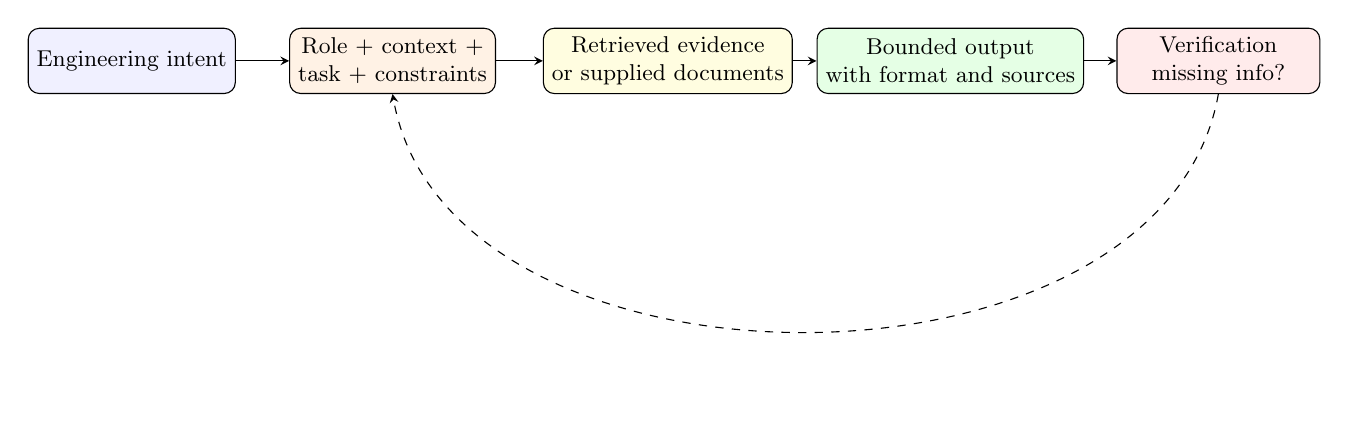
\begin{tikzpicture}[>=stealth,font=\small, scale=0.92, transform shape]
        \tikzset{box/.style={draw, rounded corners, minimum width=2.8cm, minimum height=0.9cm, align=center}}
        \node[box, fill=blue!6] (intent) at (0,0) {Engineering intent};
        \node[box, fill=orange!10] (schema) at (3.6,0) {Role + context +\\task + constraints};
        \node[box, fill=yellow!12] (evidence) at (7.4,0) {Retrieved evidence\\or supplied documents};
        \node[box, fill=green!10] (output) at (11.3,0) {Bounded output\\with format and sources};
        \node[box, fill=red!8] (check) at (15.0,0) {Verification\\missing info?};
        \draw[->] (intent) -- (schema);
        \draw[->] (schema) -- (evidence);
        \draw[->] (evidence) -- (output);
        \draw[->] (output) -- (check);
        \draw[dashed,->] (check.south) to[out=-100,in=-80] (schema.south);
    \end{tikzpicture}
    \caption{Prompt engineering as workflow design. A reliable prompt does not just ask for an answer; it structures role, evidence, output format, and verification behavior.}
    \label{t16fig:prompt_workflow}
\end{figure}

The point of Figure~\ref{t16fig:prompt_workflow} is that prompt engineering is closer to interface design than to incantation. The prompt helps organize evidence, task specification, and verification into a lightweight program-like workflow.

\section{Direct LLM Applications in Engineering Work}

We can now summarize the most important direct applications of LLMs before full frontier autonomy enters the picture.

\subsection{Document-Centered Applications}

These include:
\begin{itemize}
    \item summarizing long reports or standards;
    \item extracting assumptions, risks, and action items;
    \item comparing revisions of specifications or memos;
    \item generating draft technical narratives from structured inputs; and
    \item supporting question answering over project archives.
\end{itemize}

These are often the first high-value applications because they directly target knowledge bottlenecks rather than final design authority.

\subsection{Coding and Programming Assistance}

LLMs are also becoming practical front ends for programming. Coding assistants can:
\begin{itemize}
    \item explain unfamiliar codebases;
    \item draft scripts for parsing, analysis, or visualization;
    \item translate intent into regular expressions, SQL, or Python;
    \item propose tests, refactors, or documentation; and
    \item help navigate multi-file code repositories more quickly.
\end{itemize}

Students should see this as more than autocomplete. Modern coding tools increasingly combine language understanding, repository search, structured output, and tool integration.

\begin{figure}[ht]
    \centering
    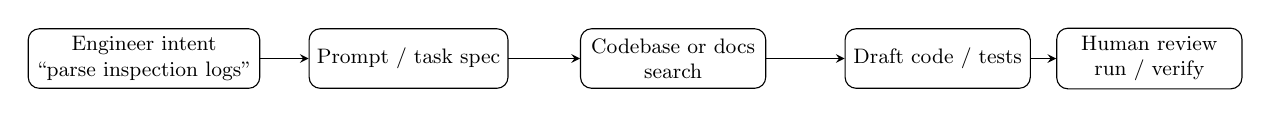
\begin{tikzpicture}[>=stealth,font=\small, scale=0.84, transform shape]
        \tikzset{box/.style={draw, rounded corners, minimum width=2.8cm, minimum height=0.9cm, align=center}}
        \node[box] (intent) at (0,0) {Engineer intent\\``parse inspection logs''};
        \node[box] (prompt) at (4,0) {Prompt / task spec};
        \node[box] (search) at (8,0) {Codebase or docs\\search};
        \node[box] (draft) at (12,0) {Draft code / tests};
        \node[box] (review) at (15.2,0) {Human review\\run / verify};
        \draw[->] (intent) -- (prompt);
        \draw[->] (prompt) -- (search);
        \draw[->] (search) -- (draft);
        \draw[->] (draft) -- (review);
    \end{tikzpicture}
    \caption{A direct coding-assistant workflow. This remains a human-directed engineering pipeline: natural-language intent is translated into search, draft generation, and explicit verification rather than unconstrained autonomy.}
    \label{t16fig:coding_workflow}
\end{figure}

\subsection{Examples of AI-Native Coding Front Ends}

Tools such as GitHub Copilot, Claude Code, and OpenCode represent a broader change in the software interface. The user increasingly describes an objective in language, and the tool translates that into code search, code generation, edits, verification steps, or planning assistance.

This is why the phrase ``language is software'' is becoming more than a metaphor. In many workflows, natural language now acts as a control layer over computational systems.

\begin{ex-box}
\textbf{Engineering coding example.} A civil engineering student wants to compare sensor drift before and after recalibration. Instead of manually building the script from scratch, the student may ask the assistant to inspect the CSV schema, write a cleaning function, generate a plotting routine, and explain the assumptions in the analysis. The useful output is not just the code. It is the accelerated movement from problem description to runnable workflow.
\end{ex-box}

\section{Language as Programming, Language as Software}

This chapter naturally leads to a broader conceptual shift. In classical software engineering, programming usually means writing formal code in languages such as Python, C++, or MATLAB. In modern LLM workflows, natural language increasingly acts as a specification layer.

This does not mean natural language replaces formal software. It means that natural language now controls, configures, and composes more of the computational workflow than before. A prompt can define a role, call for a retrieval step, request a schema, invoke a tool, and constrain the output. That is not identical to a formal program, but it is increasingly program-like.

\begin{def-box}
\textbf{Working thesis.} In modern AI workflows, language is becoming a software interface. Formal code still executes the work, but natural language increasingly specifies objectives, constraints, orchestration, and interaction patterns.
\end{def-box}

This is especially important for engineering because engineering work is already mediated by language: requirements, standards, contracts, reports, and code comments are all part of the computational ecosystem. LLM systems make that language more executable.

\section{Why Topic 17 Must Go Further}

At this point, the natural next question is: if prompts can orchestrate steps, if retrieval can ground answers, if ReAct can interleave thought and action, and if coding assistants can navigate tools, what happens when those pieces are combined into larger autonomous workflows?

That question belongs to Topic 17. There we will look at the frontier layer: modern agentic workflows, skills, multi-step tool use, and representative systems such as automated research assistants. Only after that does the human-in-the-loop issue become fully concrete. The more capable the workflow, the more urgent the questions of oversight, trust, accountability, and engineering responsibility.

\begin{alert-box}
\textbf{Transition to Topic 17:} Topic 16 showed that useful AI engineering begins well before full autonomy. Topic 17 will ask what changes when these first-generation workflows become persistent, tool-using, multi-step systems that look increasingly agentic.
\end{alert-box}

\end{document}
